\documentclass[border=4pt]{standalone}
% Shared typography and colours for the standalone figures.
\usepackage{unicode-math}
\setmainfont{TeX Gyre Termes}
\setmathfont{TeX Gyre Termes Math}
\usepackage{tikz}
\usetikzlibrary{arrows.meta,positioning,calc,decorations.pathreplacing}
\usepackage{pgfplots}
\pgfplotsset{compat=1.18}

% One colour per element or subsystem. Record the mapping in
% the working repository conventions and use it identically in every figure.
\definecolor{elemA}{HTML}{1F5FA8}
\definecolor{elemB}{HTML}{B8461B}
\definecolor{elemC}{HTML}{2E7D32}
\definecolor{elemD}{HTML}{6A4C93}
\definecolor{frameline}{HTML}{555555}

\begin{document}
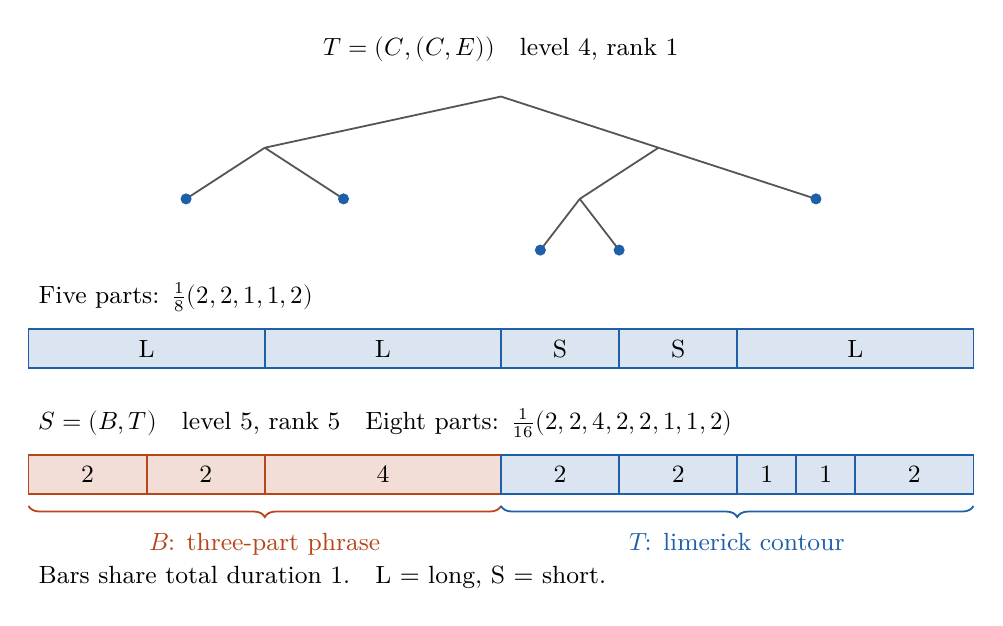
\begin{tikzpicture}[font=\small,line width=.65pt]
\node at (6,1.7) {$T=(C,(C,E))$\quad level 4, rank 1};
\coordinate (r) at (6,1.1);
\coordinate (l) at (3,.45); \coordinate (rr) at (8,.45);
\coordinate (rl) at (7,-.2);
\draw[frameline] (r)--(l) (r)--(rr) (l)--(2,-.2) (l)--(4,-.2)
 (rr)--(rl) (rr)--(10,-.2) (rl)--(6.5,-.85) (rl)--(7.5,-.85);
\foreach \x/\y in {2/-.2,4/-.2,6.5/-.85,7.5/-.85,10/-.2}
 \fill[elemA] (\x,\y) circle (2pt);
\node[anchor=west] at (0,-1.45) {Five parts: $\frac18(2,2,1,1,2)$};
\foreach \a/\b/\lab in {0/3/L,3/6/L,6/7.5/S,7.5/9/S,9/12/L} {
 \fill[elemA!16] (\a,-2.35) rectangle (\b,-1.85);
 \draw[elemA] (\a,-2.35) rectangle (\b,-1.85);
 \node at ({(\a+\b)/2},-2.10) {\lab};
}
\node[anchor=west] at (0,-3.05) {$S=(B,T)$\quad level 5, rank 5\quad Eight parts: $\frac1{16}(2,2,4,2,2,1,1,2)$};
\foreach \a/\b/\lab in {0/1.5/2,1.5/3/2,3/6/4} {
 \fill[elemB!18] (\a,-3.95) rectangle (\b,-3.45);
 \draw[elemB] (\a,-3.95) rectangle (\b,-3.45);
 \node at ({(\a+\b)/2},-3.70) {\lab};
}
\foreach \a/\b/\lab in {6/7.5/2,7.5/9/2,9/9.75/1,9.75/10.5/1,10.5/12/2} {
 \fill[elemA!16] (\a,-3.95) rectangle (\b,-3.45);
 \draw[elemA] (\a,-3.95) rectangle (\b,-3.45);
 \node at ({(\a+\b)/2},-3.70) {\lab};
}
\draw[decorate,decoration={brace,mirror,amplitude=4pt},elemB] (0,-4.1)--(6,-4.1)
 node[midway,below=6pt] {$B$: three-part phrase};
\draw[decorate,decoration={brace,mirror,amplitude=4pt},elemA] (6,-4.1)--(12,-4.1)
 node[midway,below=6pt] {$T$: limerick contour};
\node[anchor=west] at (0,-5) {Bars share total duration 1.\quad L = long, S = short.};
\end{tikzpicture}
\end{document}
